
\documentclass{uofa-eng-assignment}

\usepackage{lipsum}
\usepackage{amsmath}
\usepackage{xcolor}
%\usepackage{algorithm}
\usepackage{algorithm}
\usepackage{tabularx}
\usepackage{hyperref}
%\usepackage[algo2e]{algorithm2e} 
%\usepackage{arevmath}     % For math symbols
\usepackage[noend]{algpseudocode}
\usepackage{tikz}
\usetikzlibrary{automata, arrows.meta, positioning}

\newcommand*{\name}{Chaitanya Kadali, Sai Ram Naik}
\newcommand*{\id}{2019CS50435, 2019CS10340}
\newcommand*{\course}{ Database Management  (COL362) }
\newcommand*{\assignment}{Milestone-1}

\begin{document}

\maketitle

\noindent The project we are doing is almost similar to twitter application. Our application project "Freak" also has users and they can follow other users, or tweet and also report tweets by other users. We also have an option of liking tweets by other person. Our application consists of 4 main entity sets i.e Users, Tweets, Links and Hashtags.  

\noindent The following sections contain ER Diagram, And an overview of the modified database we created from the database we used.

\begin{center}
    \underline{\textbf{ER Diagram}}
\end{center}


        \begin{figure}[h]
        \begin{center}
            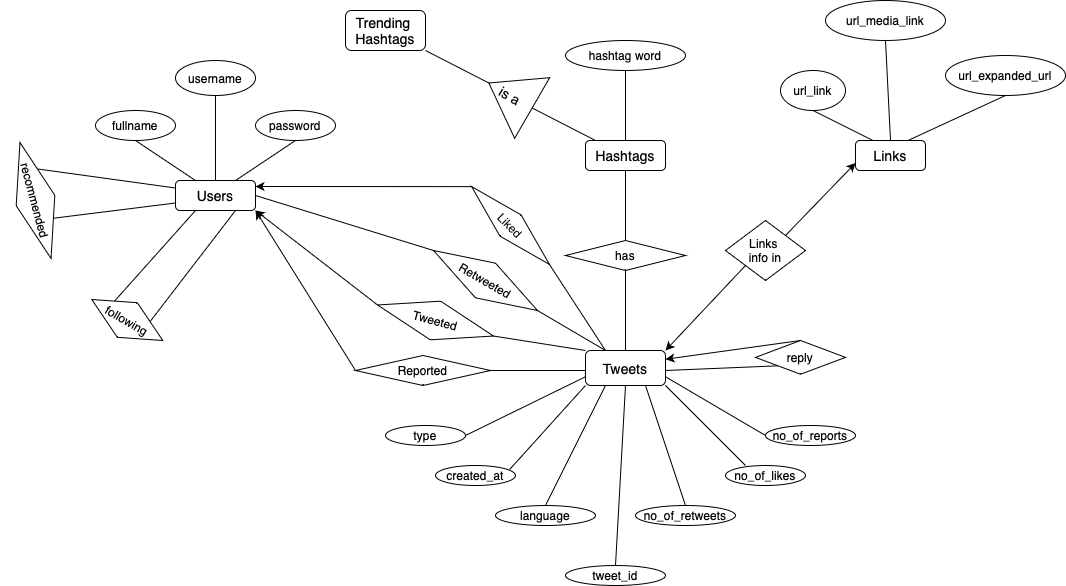
\includegraphics[scale=0.45]{erdiag.png}
            \caption{ER Diagram}
        \end{center}
        \end{figure}

\clearpage

\begin{center}
    \underline{\textbf{Main Tables in our Database}}
\end{center}

\noindent The data for this project is taken from \href{https://data.mendeley.com/datasets/7ph4nx8hnc/1}{https://data.mendeley.com/datasets/7ph4nx8hnc/1}

\noindent Eventhough this data is collected during the pandemic period and the tweets are related to covid pandemic, this still contains the users personal details and also large enough to create a database social network application. Also we would like to add login and create account options, and this further increases our database size.


\begin{center}
        \begin{tabular}{|c | c|}
            \hline
            Entity sets & Attributes \\ 
            \hline 
            Tweets & Tweet\_id \\ 
             & Type \\
             & Created\_at \\
             & No\_of\_likes \\
             & No\_of\_retweets \\
             & No\_of\_reports \\
             & Language \\
           \hline 
            Users & fullname \\
             & username \\
             & password \\
            \hline 
            Links &  Tweet\_url (link of the tweet)\\
             & Media\_url (Link of the media in the tweet if exists) \\
             & url\_expanded\_url (url in the tweet if exists) \\
            \hline 
            Hashtags & Hashtag word \\
            \hline 
        \end{tabular}
\end{center}

\vspace{2cm}
\begin{center}
    \underline{\textbf{Refining}}
\end{center}

\noindent The original raw data from the link given above consists of 8 tables. And we have extracted 6 tables for our project purpose. Those tables are listed below.

\begin{enumerate}
    \item[1.] \textbf{Users} : contains all the personal details like username, fullname, password of a person. This information is extracted from Tw.nodes.csv 
    \item[2.] \textbf{Tweets} : contains the information about the tweets. This information is extracted by Joining User.And.Type.csv and Tw.Date.Lang.csv 

    \item[3.] \textbf{Links} : contains all the information about the links. This information is extracted from Links.Media.Tweets.csv

    \item[4.] \textbf{Hashtags} : contains all the information about the Hashtags. This information is extracted from Hashtags.csv

    \item[5.] \textbf{Followers} : contains all the information about the followers of a person. This information is extracted by self joining of Tw.Edges.csv 

    \item[6.] \textbf{Edges} : extracted from Edges.csv 

    \begin{center}
    \begin{tabular}{|c | c| c |  c|}
        \hline 
        Table name & No.of Rows & Size before Refining & Size after Refining \\
        \hline 
        Users & 3565514 & 3565514 & 3565514 \\
        Tweets & 8982694 & 8982694 & 8982694 \\
        Links & 8982694 & 8982694 & 8982694 \\
        Hashtags & 3239024 & 3239024 & 3239024 \\
        Followers & 921622 & 921622 & 021622 \\
        Edges & 921622 & 921622 & 921622 \\
        \hline  
    \end{tabular}
    \end{center}

\end{enumerate}

\end{document}

